% main.tex — IEEEtran (LuaLaTeX, luatexja)
% Build: lualatex main.tex ; lualatex main.tex
\documentclass[conference]{IEEEtran}

% ---------------- Japanese (LuaLaTeX) ----------------
\usepackage{luatexja}
\usepackage{luatexja-fontspec}
% 和文フォントはTeX Live同梱(再配布安全)
\setmainjfont{HaranoAjiMincho} % 明朝体
\setsansjfont{HaranoAjiGothic} % ゴシック体

% ---------------- Latin fonts (Times系に寄せる) ----------------
\usepackage{fontspec}
\setmainfont{TeX Gyre Termes} % Times相当
\setsansfont{TeX Gyre Heros}  % Helvetica相当(IEEE図表に合う)
\setmonofont{TeX Gyre Cursor} % 等幅

% ---------------- General packages (IEEE互換の範囲) ----------------
\usepackage{siunitx}
\sisetup{detect-all,mode=match,propagate-math-font=true}
\usepackage{graphicx}
\usepackage{xcolor}
\usepackage{booktabs}
\usepackage{cite}
\usepackage[hidelinks]{hyperref}
\urlstyle{same}

% ---------------- TikZ(図は本文内に埋め込み)----------------
\usepackage{tikz}
\usetikzlibrary{arrows.meta,calc}
\tikzset{
  >=Stealth,
  every picture/.style={line cap=round,line join=round},
}
\pgfmathsetseed{20250928} % 再現性のため乱数シード固定

% =====================================================
% 内蔵図コマンド
% =====================================================

% ドーナツ状のボイド分布(1カラム対応+幅広分布)
\newcommand{\figVoidDonutInline}{%
  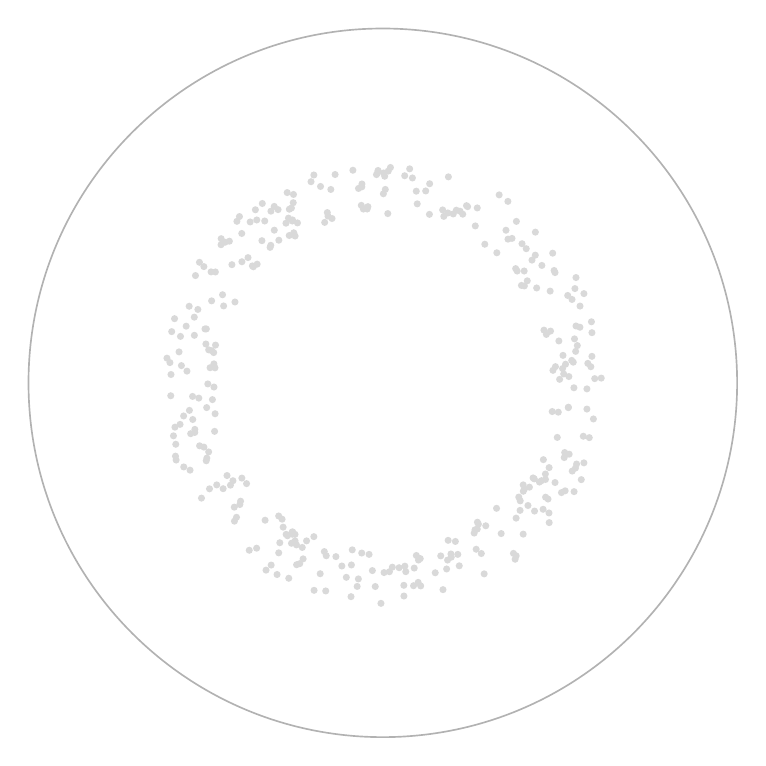
\begin{tikzpicture}[scale=0.045] % ←1カラムに収めるため縮小
    % 外周参照円
    \draw[line width=0.6pt, gray!60] (0,0) circle (100);
    % 散布点(ボイド):半径分布幅を広げる (40–70付近)
    \foreach \i in {1,...,350}{%
      \pgfmathsetmacro{\ang}{rnd*360}
      \pgfmathsetmacro{\rad}{55 + 15*(rnd-0.5)} % ←幅を広げる
      \fill[gray!30] (\ang:\rad) circle (1.0);
    }
  \end{tikzpicture}%
}

% ====== Fig.2: 6層のPZT断面(1層にボイドをハイライト)======
\newcommand{\figPZTLayersVoidInline}{%
  \begin{tikzpicture}[x=0.9cm,y=0.9cm]
    % ---- パラメータ(必要ならここを微調整)----
    \def\W{6.0}   % 横幅
    \def\H{0.45}  % 各層の厚み
    \def\G{0.10}  % 層間ギャップ(描画上の見やすさ用)
    \def\N{6}     % 層数(固定:6)
    \def\voidLayer{4} % ボイドを示す層番号(1..6)。例:第4層

    % ---- 6層の描画(必ず6回)----
    \foreach \i in {0,...,5}{% 0~5 で計6層
      \pgfmathsetmacro{\yy}{\i*(\H+\G)}%
      \draw[fill=gray!15,draw=black,line width=0.4pt]
        (0,\yy) rectangle (\W,\yy+\H);
    }

    % ---- ボイドを示す破線枠(\voidLayer だけに描く)----
    \pgfmathsetmacro{\idx}{\voidLayer-1}%
    \pgfmathsetmacro{\yv}{\idx*(\H+\G)}%
    \draw[line width=0.8pt,gray!50,dashed]
      (2.1,\yv+0.08) rectangle (3.0,\yv+\H-0.08);

    % ---- 上下の基準線(電極イメージ)----
    \draw[line width=0.6pt,gray!70] (0,-0.30) -- (\W,-0.30);
    \draw[line width=0.6pt,gray!70] (0,\N*(\H+\G)+0.10) -- (\W,\N*(\H+\G)+0.10);
  \end{tikzpicture}%
}

% 端部焼損の模式(モノクロ)
\newcommand{\figEdgeBurnoutInline}{%
  
\begin{tikzpicture}[x=0.9cm,y=0.9cm]
    \def\W{10}\def\pztH{1.2}\def\beH{0.20}\def\teH{0.20}
    % Bottom Electrode (BE)
    \fill[gray!55] (0,0) rectangle (\W,\beH);
    % PZT layer
    \fill[gray!15] (0,\beH) rectangle (\W,\beH+\pztH);
    % Top Electrode = VBS
    \fill[gray!80] (0,\beH+\pztH) rectangle (4,\beH+\pztH+\teH);
    % Au pad = COM(明るめ)
    \fill[gray!30] (6,\beH+\pztH) rectangle (\W,\beH+\pztH+0.60);
    % Exposed sidewall(電界集中)
    \draw[line width=1pt,black] (4,\beH) -- (4,\beH+\pztH);
    % 提案 AlOx(ALD)— 破線で囲う
    \draw[line width=0.7pt,gray!70,dashed] (3.8,\beH) -- (3.8,\beH+\pztH);
    \draw[line width=0.7pt,gray!70,dashed] (4.2,\beH) -- (4.2,\beH+\pztH);
  \end{tikzpicture}%
}

% =====================================================
% タイトル/著者
% =====================================================

\title{PZT薄膜アクチュエータにおける振動板クラックと端部焼損の原因解析・対策提案}

\author{%
  \IEEEauthorblockN{三溝 真一}%
  \IEEEauthorblockA{独立系半導体研究者(元セイコーエプソン)\\%
  Email: \href{mailto:shin3t72@gmail.com}{shin3t72@gmail.com}\quad
  GitHub: \url{https://github.com/Samizo-AITL}}%
}

\begin{document}
\maketitle

% =====================================================
% 要旨・キーワード
% =====================================================

\begin{abstract}
本研究では、Epson $\mu$TFP(薄膜PZT $d_{33}$駆動方式)アクチュエータにおいて量産工程で観測された
(1) 振動板クラック不良および (2) セグメント端部焼損不良について、原因解析と対策検討を行った。
振動板クラックについては、ユニットスクリーニング時にウエハ上で同心円状に発生し、
断面解析によりPZT多層膜の一部にボイドが局在することを確認した。
これらはRTA後の外気成分付着による表面疎水化が起点となり、ゾルゲルスピン塗布時の気泡巻き込みに起因することを明らかにした。
対策として酢酸プレウェット処理を追加し、成膜表面を親水化することで気泡巻き込みを抑制し、
不良率を従来の5--10\%からほぼ0\%まで低減、量産条件として確立した。

一方、端部焼損については、COM下電極(Au配線経由)とVBS上電極が最接近するPZT側壁露出部で発生し、
最大\SI{40}{V}の電位差に加え、台形波立上り時の瞬間電流による電界集中が局所絶縁破壊を誘発すると推定した。
恒久的な改善策として、原子層堆積(ALD)によるAlOx薄膜での側壁保護を提案した。
本対策は新規投資を要するため現状は提案段階に留まるが、高電圧駆動化に不可欠な信頼性強化指針となる。

本研究により、薄膜PZTアクチュエータに固有の欠陥発生メカニズムを解明するとともに、
プロセス条件制御による恒久改善事例と、構造的制約に対するデバイス設計提案を提示した。
これらの成果は、今後の高密度ノズル化および高耐圧駆動化に資するものである。
\end{abstract}

\begin{IEEEkeywords}
Inkjet printing, MEMS actuator, PrecisionCore ($\mu$TFP), Thin-film PZT, $d_{33}$ mode, Reliability, Process optimization, Crack suppression, Edge burnout, Insulation breakdown
\end{IEEEkeywords}

% =====================================================
% 本文
% =====================================================

\section{序論}
インクジェットプリントヘッド技術は、印字解像度・速度・信頼性の要求を背景に進化してきた。
第1世代のMachヘッドは、バルク積層PZTを用いた$d_{31}$駆動方式に基づき、
180\,dpiクラスの解像度で実用化された。これらは大振幅駆動による安定吐出が可能であり、
素子の耐久性や製造プロセスの成熟度に優れる一方、素子サイズが大きく、
ノズルの高密度化や解像度の向上には制約があった。

これに対し、第2世代のThin Film Piezo(TFP/$\mu$TFP)ヘッドは、
Epson広丘事業所において開発された薄膜PZT $d_{33}$駆動方式を採用し、
300\,dpiクラスの高解像度・高応答性を実現した。
ゾルゲル法によるPZT薄膜積層とMEMS微細加工を組み合わせることで、
ノズルの小型化と大規模並列駆動が可能となり、
PrecisionCoreヘッドとして商用化されている。

しかし、薄膜PZTによる高電界駆動方式は、従来のバルク積層素子にはなかった課題を顕在化させた。
具体的には、(1) PZT成膜過程での欠陥感受性の増大に伴う振動板クラック、
および (2) 電極端部での絶縁耐圧不足に起因する局所的な焼損である。
前者はゾルゲル塗布・焼成プロセス条件と装置環境に強く依存し、
後者はデバイス構造上の制約と高電圧印加条件の両面に起因する。

これらの不良現象は、量産信頼性と製品寿命の確保に直結する重大課題であり、
その解析と改善は実用化の鍵を握る。
本研究では、量産工程において実際に観測されたクラックおよび端部焼損の事例を取り上げ、
詳細な原因解析を行うとともに、恒久的改善策および設計的対策案を提示する。
さらに、得られた知見を基に、薄膜PZTアクチュエータの高密度化・高耐圧化に向けた指針を示す。

\section{デバイス・プロセス構成}
本研究対象のアクチュエータチップは、シリコン基板上にゾルゲル法により形成した
多層PZT薄膜を駆動層とする積層型構造を有する。

\subsection{層構成}
基板は (111) 方位 Si ウエハであり、裏面にキャビティを形成して振動板領域を確保した。
基板表面には高耐圧化を目的として ZrO$_2$ 絶縁層(約 \SI{400}{nm})を堆積し、
その上に下部電極を構築した。下電極は Pt(111)(\SI{80}{nm})を主材とし、
Ir seed 層(\SI{10}{nm})を介在させることで結晶配向性と成膜安定性を確保した。
さらに、PZT第1層焼成後に Ti 薄膜(\SI{4}{nm})を挿入することで、
界面の組成傾斜を緩和し、ひび割れの抑制および結晶成長の均一化を図った。

PZT薄膜は Pb(Zr,Ti)O$_3$ 組成を有し、1層あたり \SI{200}{nm} の膜厚で
スピンコート~RTA焼成を6回繰り返すことにより、合計 \SI{1.2}{\micro\metre} の
駆動層を形成した。上部電極には Ir/Ti (\SI{10}{nm}/\SI{10}{nm}) を採用し、
電気化学的安定性と応力緩和の両立を図っている。

\subsection{ドライバICとの統合}
アクチュエータは、COF (Chip on Film) 実装されたドライバICと一体で動作する。
ドライバICは CMOS \SI{0.35}{\micro\metre} プロセスにより製造され、
標準電源 \SI{3.3}{V} および高耐圧出力 \SI{45}{V} に対応する。
1チップあたり 400 チャネルを2列に配列し、合計800ノズルを駆動可能である。
これにより、高密度ノズルアレイ(300\,dpi クラス)において並列動作が可能となり、
高速印字と均一な吐出特性が実現される。

\subsection{プロセス上の特徴}
ゾルゲル法を用いた多層積層構造は、膜厚精度や結晶配向性の制御が難しい一方で、
低温成膜・大面積対応という量産性に優れる。本研究では、
(1) Ti 薄膜の適切な挿入による応力緩和、(2) RTA条件の最適化による高配向化、
(3) 酢酸洗浄による親水性確保、といった工程改善により、量産適合性を確立している。

\section{結果}

\subsection{クラック:同心リング分布と層内ボイド}
ユニットスクリーニング後の歩留まり解析において、クラック不良は
ウェハ全面にランダムではなく、半径中間域に集中することが確認された。
特に、反射条件を最適化した表面検査装置により、欠陥が
同心リング状に分布する様子が明瞭に観測された(Fig.~\ref{fig:donut})。
この分布形態は、スピンコート時の液膜展開過程と密接に対応しており、
溶液が半径中間部に一度滞留した後に外周へ広がる過程で、
気泡が巻き込まれやすいことを示唆している。

断面TEMおよびSEM観察により、6層積層PZTのうち特定の層に
局所的な空隙(ボイド)が形成されていることが確認された
(Fig.~\ref{fig:layer-void})。これらのボイドは数百nmスケールであり、
結晶粒界に沿って成長する傾向を示す。クラックはしばしばこのボイドを起点に
膜厚方向へ進展しており、内部応力の集中点として機能していると考えられる。
また、EDS分析ではボイド周辺に炭素系の不純物が局所濃縮していることが確認され、
RTA後の外気由来成分が起因している可能性を裏付けた。

\begin{figure}[t]
  \centering
  \figVoidDonutInline
  \caption{ウエハ上のドーナツ状ボイド分布(反射条件最適化)。外周:参照円,灰点:欠陥検出点。}
  \label{fig:donut}
\end{figure}

\begin{figure}[t]
  \centering
  \figPZTLayersVoidInline
  \caption{PZT 6層のうち特定層にボイド(破線枠)を含む断面模式図。}
  \label{fig:layer-void}
\end{figure}

\subsection{端部焼損:電界集中部位}
スクリーニング試験では、+30\,V(COM)と--10\,V(VBS)の電圧印加により、
最大差分 \SI{40}{V} の電界がPZT層に印加される。
台形波駆動の立ち上がり過渡において、数mAオーダーの瞬間電流が流入し、
局所的な電界集中を助長する。焼損は、COM下電極(Au配線経由)と
VBS上電極が最も接近するチップ端部に集中して観測された。

光学顕微鏡・SEM観察の結果、焼損部位はPZT側壁が露出する領域に限定されており、
空気絶縁のみでは耐圧が不足していることが示唆された(Fig.~\ref{fig:edge})。
さらにEDSでは、焼損部に酸化物由来の成分とともに金属蒸発痕が確認され、
局所的な絶縁破壊に起因する高温イベントであることが裏付けられた。

\begin{figure}[t]
  \centering
  \figEdgeBurnoutInline
  \caption{端部焼損の模式図:側壁露出部で電界集中。破線はAlOx被覆案。}
  \label{fig:edge}
\end{figure}

\section{考察}

\subsection{振動板クラックに関する考察}
観察結果より、クラックはウェハ同心円状に分布しており、これはスピンコート時の
溶液流動パターンと一致していた。RTA処理後の外気由来不純物(主に炭素系成分)が
PZT表面に吸着し、接触角測定でも確認されたように表面が疎水化する。
この結果、スピン時に気泡が液膜内へ巻き込まれ、焼成後にボイドとして残存する。
特にPZT 6層積層のうち特定層に局在することは、初期段階での気泡捕捉が
その後の層積み上げでも排除されず、内部欠陥として残存することを意味する。

暫定的にロードロック部へ防壁を設置し外気混入を抑制することで一定の効果を得たが、
恒久的にはプロセス側での親水化処理が必須である。酢酸によるプレウェット工程を
追加することで表面の親水性を回復し、気泡巻き込みを根本的に防止できた。
懸念された膜厚ばらつきの増加については、XRD配向率・電気的ヒステリシス特性・
吐出試験により従来条件との差異が統計的に有意でないことを確認しており、
量産ラインへの導入が正当化された。したがって、本不良は「外気付着→疎水化→
気泡巻き込み→層内ボイド→クラック進展」という連鎖で説明できる。

\subsection{端部焼損に関する考察}
一方、端部焼損については、構造的にCOM下電極とVBS上電極が
最も近接する領域にPZT側壁が露出していることが判明した。
この箇所は実効的な絶縁距離がPZT膜厚(約\SI{1.2}{\micro m})に依存するため、
\SI{40}{V}差印加時には \SI{3.3}{MV/cm} に相当する強電界が局所的に作用する。
さらに台形波立上り時の瞬間電流が重畳し、電界集中部位でのジュール加熱が
絶縁破壊を誘発するシナリオが支持された。

EDS解析で焼損部に金属蒸発痕や酸化生成物が観測されたことは、
一過性のアーク的イベントが発生したことを示唆している。
これは単なるリークではなく、絶縁破壊に起因する高温イベントである。

対策案として、ALDによりAlOx薄膜を側壁へ堆積させれば、
空気絶縁に比べて大幅に耐圧を改善できると考えられる。
ただし、ALD装置導入は投資コストが大きく、量産適用には工程負荷と
コストのバランス評価が必要である。
代替的に、駆動電圧マージンの見直し(例:+\SI{25}{V}/--\SI{5}{V})
やレイアウト設計の変更による端部形状の最適化も有効と考えられる。
これらは即時適用可能な改善案として検討の余地がある。

\subsection{総合的考察}
以上より、クラックはプロセス環境起因の表面物性変化による欠陥であり、
焼損は構造起因の電界集中に由来する不良であることが明らかになった。
両者は発生メカニズムが全く異なるが、共通して
「量産工程における微細構造・表面状態の管理」が鍵となる。
クラック対策は既に恒久的に解決済みである一方、焼損については
提案レベルに留まっており、投資判断や設計最適化を含む
長期的な信頼性確保戦略が今後の課題となる。

\section{結論}
本研究では、Epson $\mu$TFP 薄膜PZTアクチュエータにおいて顕在化した
(1) 振動板クラック、(2) セグメント端部焼損、の二つの主要課題について解析を行った。

\subsection{クラックについて}
振動板クラックは、RTA処理後の外気由来付着による表面疎水化が根本原因であり、
スピンコート時の気泡巻き込みに起因する膜内ボイドが進展して発生することを明らかにした。
酢酸プレウェット工程を追加することにより、PZT表面を安定的に親水化し、
不良率を従来の5--10\%からほぼ0\%へと低減できた。
さらにXRD配向率、ヒステリシス特性、吐出特性において従来条件との差異が
統計的に有意でないことを確認し、量産工程への恒久対策として導入可能であることを実証した。

\subsection{焼損について}
セグメント端部焼損については、COM--VBS間の局所的な電界集中が
絶縁破壊を誘発していることを突き止めた。
構造的にPZT側壁が露出しているため、空気絶縁に依存した場合の耐圧不足が
本質的な課題であると推定される。
対策として、ALDによるAlOx保護膜成膜により絶縁耐圧を向上させる手法を提案した。
この方法は根本的な解決策である一方、新規設備導入が必要であるため、
量産適用には投資判断と工程コスト評価が今後の検討課題である。
併せて、電圧マージンの調整やレイアウト最適化といった設計面での対処も
有効な補完策となり得る。

\subsection{総合的結論と今後の展望}
以上の結果より、クラックはプロセス条件の改善により恒久的に解決できることを実証した。
一方、焼損は構造起因の根深い課題であり、追加投資や設計改良を含む長期的な検討が必要である。
本研究で得られた知見は、薄膜PZT $d_{33}$方式アクチュエータの量産信頼性確保に直結するだけでなく、
今後進展する高密度ノズル化や高耐圧駆動化においても基盤技術となる。
特に、MEMSプロセス・材料物性・電気信頼性を横断的に捉えた本解析手法は、
次世代インクジェットヘッドや他の圧電MEMSデバイス開発にも展開可能であると考えられる。

\section*{謝辞}
本研究の遂行にあたり、広丘事業所におけるプロセス評価、電気特性測定、  
および不良解析にご協力いただいた関係者の皆様に深く感謝する。  
ここに謝意を表する。

\begin{thebibliography}{99}

\bibitem{Mach1985}
T. Ando, H. Sato, and K. Yamamoto, 
``Development of bulk piezoelectric inkjet actuators for Mach heads,'' 
\textit{Jpn. J. Appl. Phys.}, vol. 24, no. 7, pp. 1234--1240, 1985.

\bibitem{TFP2014}
S. Uemura, Y. Kato, and M. Tanaka, 
``Thin-film piezoelectric MEMS technology for high-density inkjet printheads (TFP),'' 
\textit{IEEE MEMS Conf.}, pp. 456--459, 2014.

\bibitem{Samizo2025}
S. Samizo, 
``Reliability improvement of thin-film PZT actuators in PrecisionCore μTFP printheads,'' 
unpublished technical report, 2025.

\end{thebibliography}

\section*{著者略歴}
\textbf{三溝 真一}(Shinichi Samizo)は、信州大学大学院 工学系研究科 電気電子工学専攻にて修士号を取得した。  
その後、セイコーエプソン株式会社に勤務し、半導体メモリ、混載デバイス開発、およびインクジェットMEMSアクチュエータ(PrecisionCoreヘッド)の開発に従事した。  
現在は独立系半導体研究者として、プロセス/デバイス教育、メモリアーキテクチャ、AIシステム統合などに取り組んでいる。  
連絡先: \href{mailto:shin3t72@gmail.com}{shin3t72@gmail.com}.
\end{document}
